%
% Complete documentation on the extended LaTeX markup used for Insight
% documentation is available in ``Documenting Insight'', which is part
% of the standard documentation for Insight.  It may be found online
% at:
%
%     http://www.itk.org/

\documentclass{InsightArticle}


%%%%%%%%%%%%%%%%%%%%%%%%%%%%%%%%%%%%%%%%%%%%%%%%%%%%%%%%%%%%%%%%%%
%
%  hyperref should be the last package to be loaded.
%
%%%%%%%%%%%%%%%%%%%%%%%%%%%%%%%%%%%%%%%%%%%%%%%%%%%%%%%%%%%%%%%%%%
\usepackage[dvips,
bookmarks,
bookmarksopen,
backref,
colorlinks,linkcolor={blue},citecolor={blue},urlcolor={blue},
]{hyperref}
% to be able to use options in graphics
\usepackage{graphicx}
% for pseudo code
\usepackage{listings}
% subfigures
\usepackage{subfigure}


%  This is a template for Papers to the Insight Journal. 
%  It is comparable to a technical report format.

% The title should be descriptive enough for people to be able to find
% the relevant document. 
\title{Image mask adaptor for pixel order independent filters}

% Increment the release number whenever significant changes are made.
% The author and/or editor can define 'significant' however they like.
\release{0.00}

% At minimum, give your name and an email address.  You can include a
% snail-mail address if you like.
\author{Richard Beare}
\authoraddress{Department of Medicine, Monash University, Australia.}

\begin{document}
\maketitle

\ifhtml
\chapter*{Front Matter\label{front}}
\fi


\begin{abstract}
\noindent
It is sometimes useful to apply a filter to a region defined by a
mask. This article introduces a simple ``mask adaptor'' filter that
allows this type of operation to be tested easily. It is applicable to
filters that do not need any pixel location information, such as
histogram operations, which can't necessarily be achieved by simple
masking approaches.
% The abstract should be a paragraph or two long, and describe the
% scope of the document.
\end{abstract}

\tableofcontents

\section{Introduction}
 The application that inspired this filter was Otsu thresholding
 applied to a specific region of the image, with the rest of the image
 being ignored.Simply masking the image and applying an Otsu threshold
 does not give the same result because the mask operation introduces a
 large number of zeros that influences histogram based
 computations. This filter, which is loosely termed a ``mask adaptor''
 simply copies all pixels defined by a mask to a temporary one
 dimensional image, applies a user defined pipeline and copies the
 results back to the correct image format. This procedure probably
 breaks streaming rules and may only be useful for histogram
 operations.

 The most recent versions of this packages can be obtained from
 \url{http://voxel.jouy.inra.fr/darcsweb/}\footnote{ The most recent
 versions can be obtained using darcs \cite{DarcsWebSite} with the
 command {\em darcs get
 http://voxel.jouy.inra.fr/\\darcs/contrib-itk/maskAdaptor}}
\section{Usage}
The new filter is called the {\em itkMaskAdaptorImageFilter} and can
be used as follows\footnote{This code is in check.cxx, included in the
distribution}. This example demonstrates separating the background
into original and padded regions, which is difficult to do using
histogram operations applied to the entire image.
\small \begin{verbatim}
#include "itkImageFileReader.h"
#include "itkImageFileWriter.h"
#include "itkCommand.h"
#include <itkBinaryThresholdImageFilter.h>

#include "itkOtsuMultipleThresholdsImageFilter.h"
#include "itkMaskAdaptorImageFilter.h"

int main(int, char * argv[])
{
  const int dim = 2;

  typedef unsigned char PType;
  typedef itk::Image< PType, dim > IType;

  typedef itk::ImageFileReader< IType > ReaderType;
  ReaderType::Pointer reader = ReaderType::New();
  reader->SetFileName( argv[1] );

  typedef itk::BinaryThresholdImageFilter<IType, IType> ThreshType;
  ThreshType::Pointer thresh = ThreshType::New();
  thresh->SetInput(reader->GetOutput());
  thresh->SetUpperThreshold(50);
  thresh->SetInsideValue(1);
  thresh->SetOutsideValue(0);

  typedef itk::OtsuMultipleThresholdsImageFilter<IType, IType> OtsuType;
  OtsuType::Pointer filter = OtsuType::New();
  filter->SetInput(reader->GetOutput());
  filter->SetNumberOfThresholds(2);

  typedef itk::ImageFileWriter< IType > WriterType;
  WriterType::Pointer writer = WriterType::New();
  writer->SetInput( filter->GetOutput() );
  writer->SetFileName( argv[2] );
  writer->Update();

  // now for the masked version
  typedef itk::MaskAdaptorImageFilter<IType, IType, IType> MaskAdaptorType;
  typedef itk::OtsuMultipleThresholdsImageFilter<MaskAdaptorType::InternalInputImageType, MaskAdaptorType::InternalOutputImageType> MaskOtsuType;

  MaskAdaptorType::Pointer masker = MaskAdaptorType::New();
  MaskOtsuType::Pointer maskotsu = MaskOtsuType::New();
  maskotsu->SetNumberOfThresholds(1);
  masker->SetFilter(maskotsu);
  masker->SetInput(reader->GetOutput());
  masker->SetMaskImage(thresh->GetOutput());
  masker->SetDefaultValue(0);

  writer->SetInput( masker->GetOutput() );
  writer->SetFileName( argv[3] );
  writer->Update();

  return 0;
}
\end{verbatim} \normalsize

The first part of the code uses a standard thresholding operation to
generate a mask of all the background region. We then apply standard
Otsu thresholding to the entire image and the region defined by the
mask. The latter requires declaring the Otsu threshold using the
internal image types defined by the MaskAdaptorType.

Results of the various steps are shown in Figures \ref{mask} and
\ref{maskotsu}. 

\begin{figure}[htbp]
\centering
\includegraphics{cthead1}
\caption{The input image.\label{cthead1}}
\end{figure}

\begin{figure}[htbp]
\centering
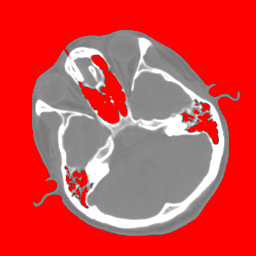
\includegraphics{mask_overlay}
\caption{The mask defining the region to which Otsu thresholding is applied.\label{mask}}
\end{figure}

\begin{figure}[htbp]
\centering
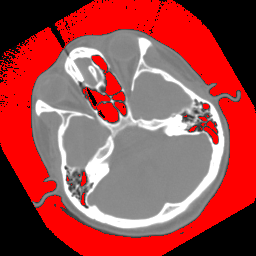
\includegraphics{mask_otsu}
\caption{The threshold calculated within the mask region. The padded region is separated from the original background.\label{maskotsu}}
\end{figure}

\section{Methods}
\begin{itemize}
\item {\bf Set/GetFilter} : Set/Get the user defined filter applied to the masked region.
\item {\bf Set/GetMaskImage} : Set/Get the mask image.
\item {\bf Set/GetInputFilter} : Set/Get the start of a processing pipeline.
\item {\bf Set/GetOutputFilter} : Set/Get the end of a processing pipeline.
\item {\bf Set/GetDefaultValue} : Set/Get the output value where the mask is zero.
\item {\bf Set/GetPassOutsideMask} : Set/Get (boolean) whether the output is copied from the input where the mask is zero. Overrides DefaultValue.
\end{itemize}


\section{Comments}
The best strategy for implementing this filter isn't clear to me. The
necessity for allocating different buffers and copying the results of
the user defined pipeline to the output buffer means that the usual
pipeline structure isn't followed. I'm not sure how best to deal with
this, and any advice on improvements are welcome.



\bibliographystyle{plain}
\bibliography{InsightJournal,local}
\nocite{ITKSoftwareGuide}

\end{document}

